\chapter{Perancangan}
\label{chap:perancangan}

Bab ini membahas tentang perancangan untuk implementasi sistem perekaman ulang dalam SharIF-Judge. Perancangan akan dilakukan dengan mempertimbangkan aspek fungsionalitas, antarmuka pengguna, penyimpanan data, serta perubahan kode yang diperlukan pada sistem yang sudah ada.

\section{Rancangan Antarmuka}

Rancangan antarmuka sistem ini dibagi menjadi dua komponen utama yaitu sistem perekaman yang terintegrasi dengan halaman \verb|Submit| yang sudah ada dan sistem pemutaran ulang yang membutuhkan pengembangan halaman baru.

\subsection{Sistem Rekaman}
\label{sub:4:1:rekaman}

Seluruh sistem rekaman akan diimplementasikan dalam halaman Submit tidak memerlukan perubahan pada antarmuka. Gambar \ref{fig:4:1:submit} menunjukkan halaman Submit dan IDE yang sudah diimplementasikan oleh Nicholas Aditya Halim~\cite{nicholas:sharif}.

\vspace{0.75cm}

\begin{figure}[H]
    \centering
    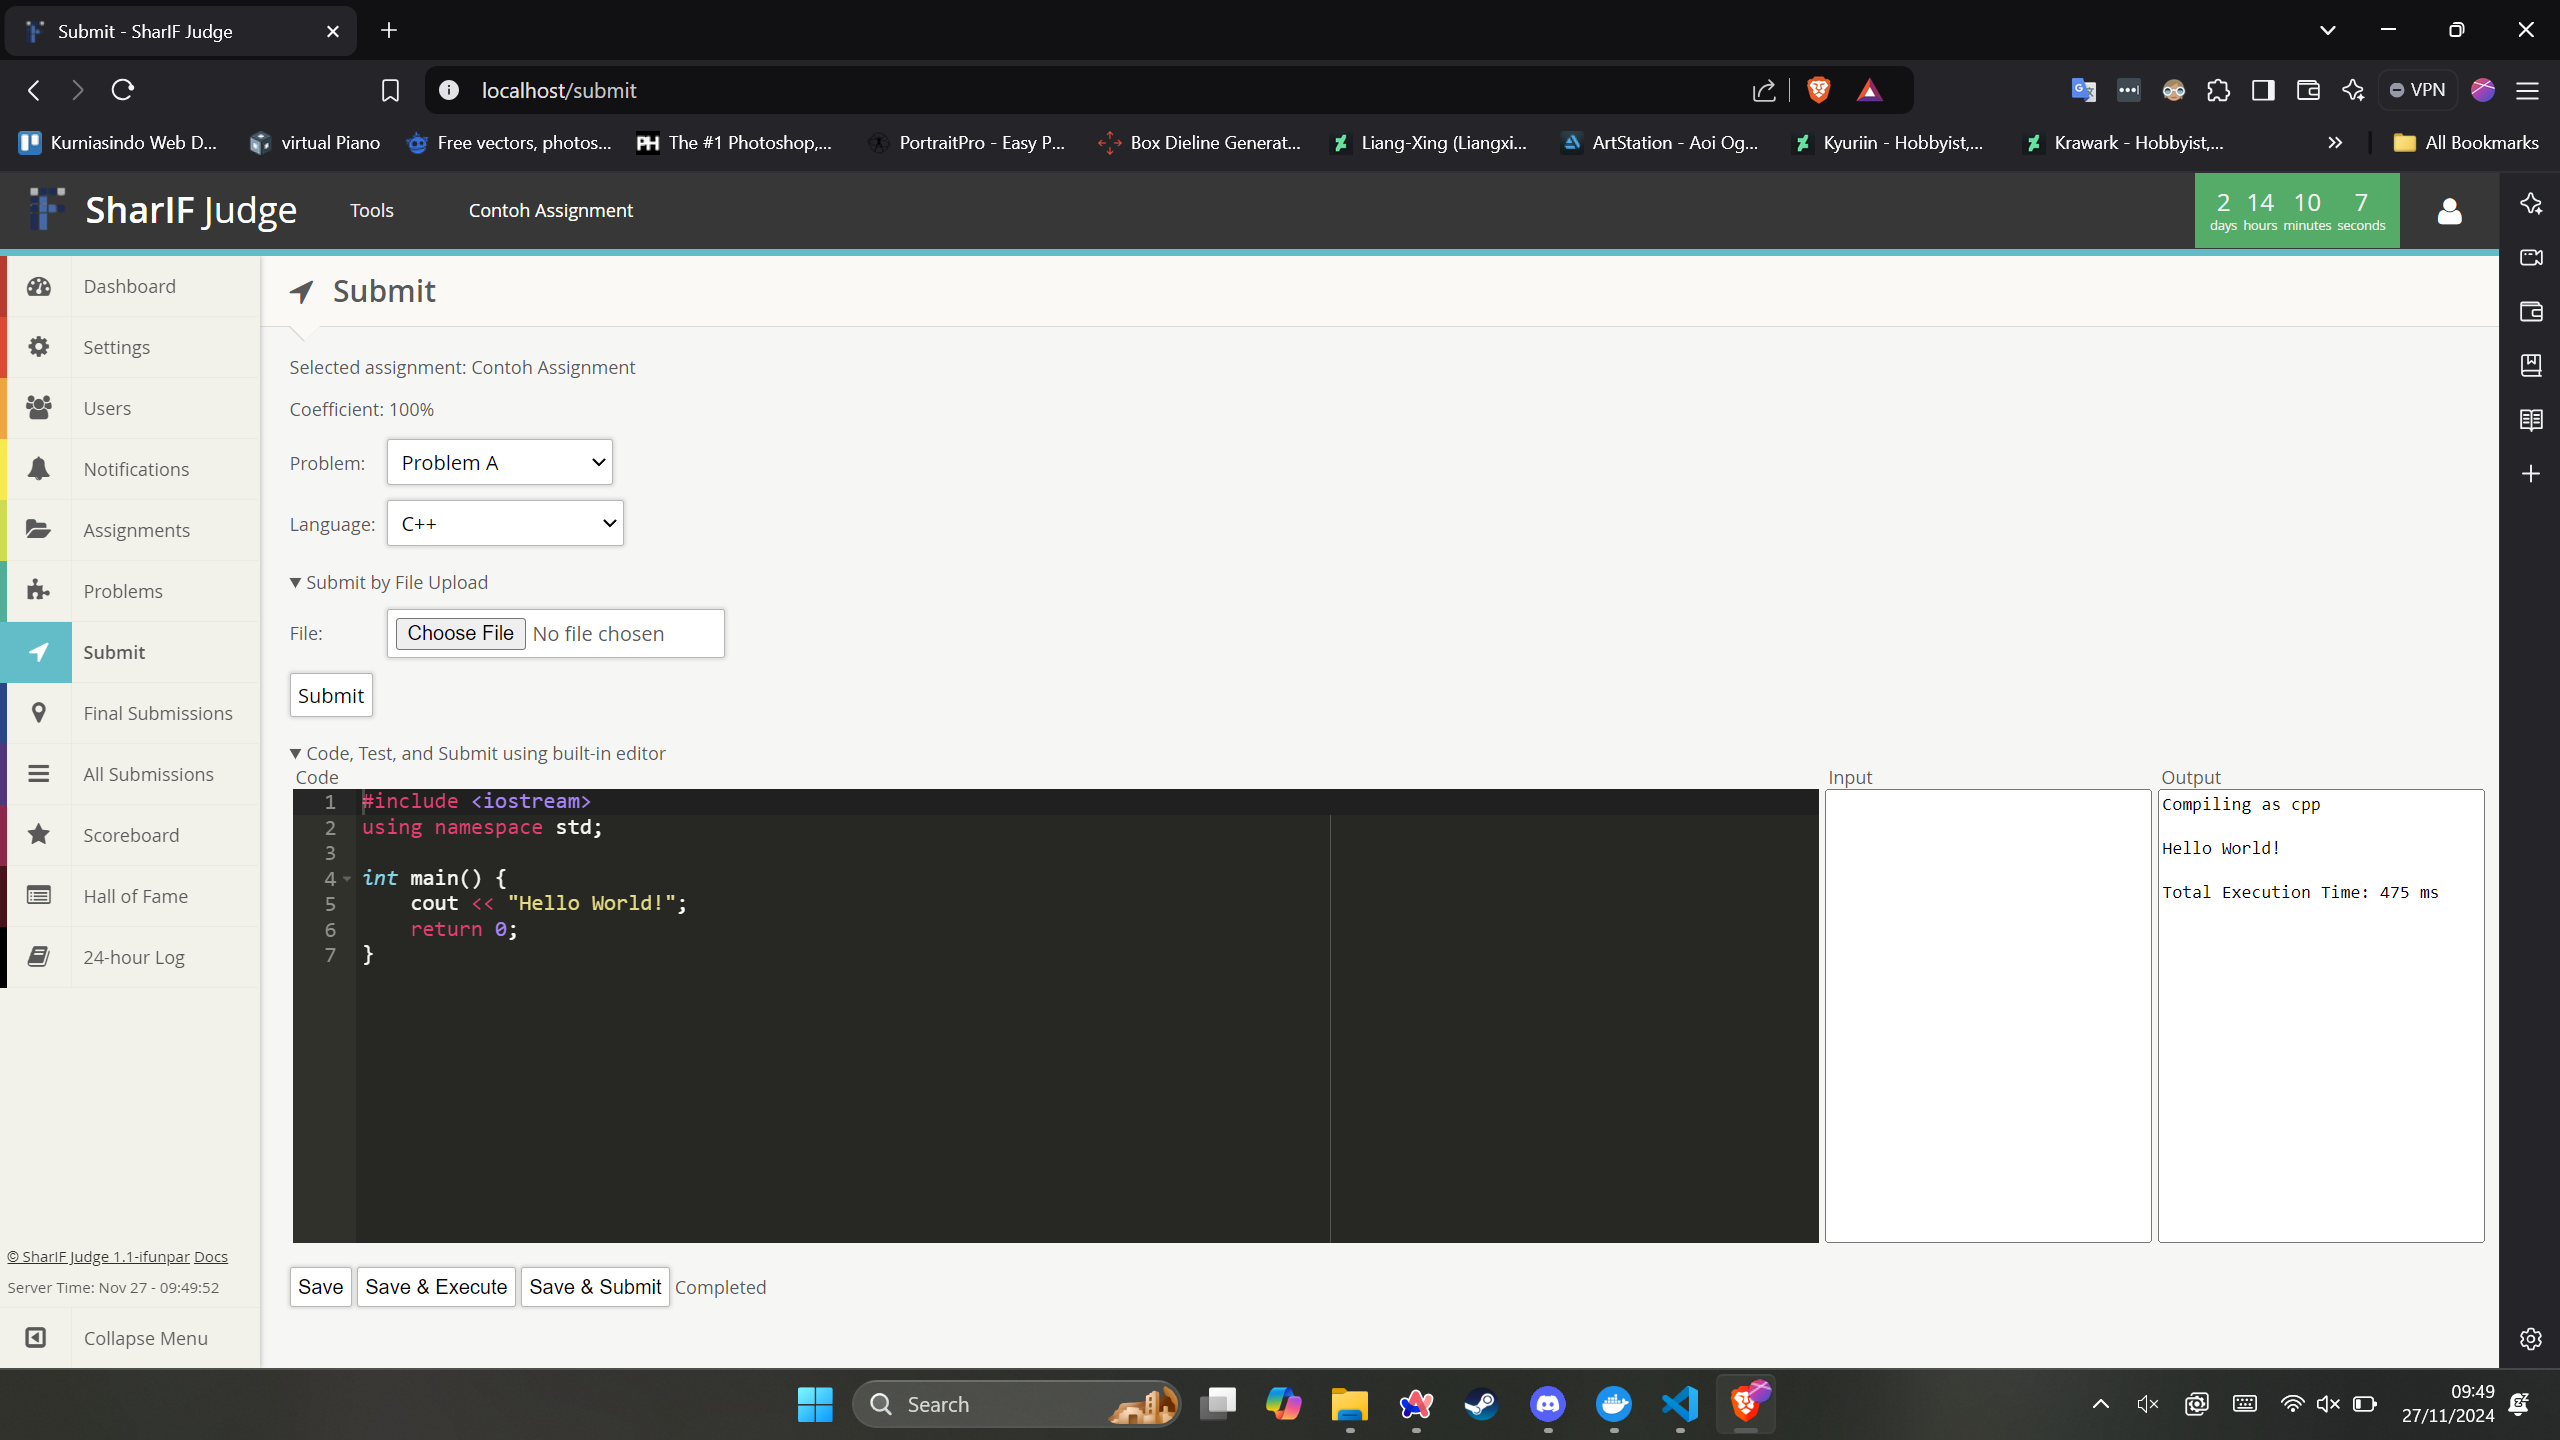
\includegraphics[width=0.85\textwidth]{views/submit.png}
    \caption{Halaman}
    \label{fig:4:1:submit}
\end{figure}

\subsection{Sistem Pemutaran ulang}
\label{sub:4:1:pemutaranulang}

Pada sistem pemutaran ulang dibutuhkan dua halaman baru yaitu halaman untuk menunjukkan daftar rekaman dalam sistem dan halaman untuk pemutaran ulang sebuah rekaman. Gambar \ref{fig:4:1:listrec} merupakan rancangan antarmuka untuk halaman daftar rekaman dan Gambar \ref{fig:4:1:rec} merupakan rancangan antarmuka untuk halaman pemutaran ulang.

\begin{figure}[H]
    \centering
    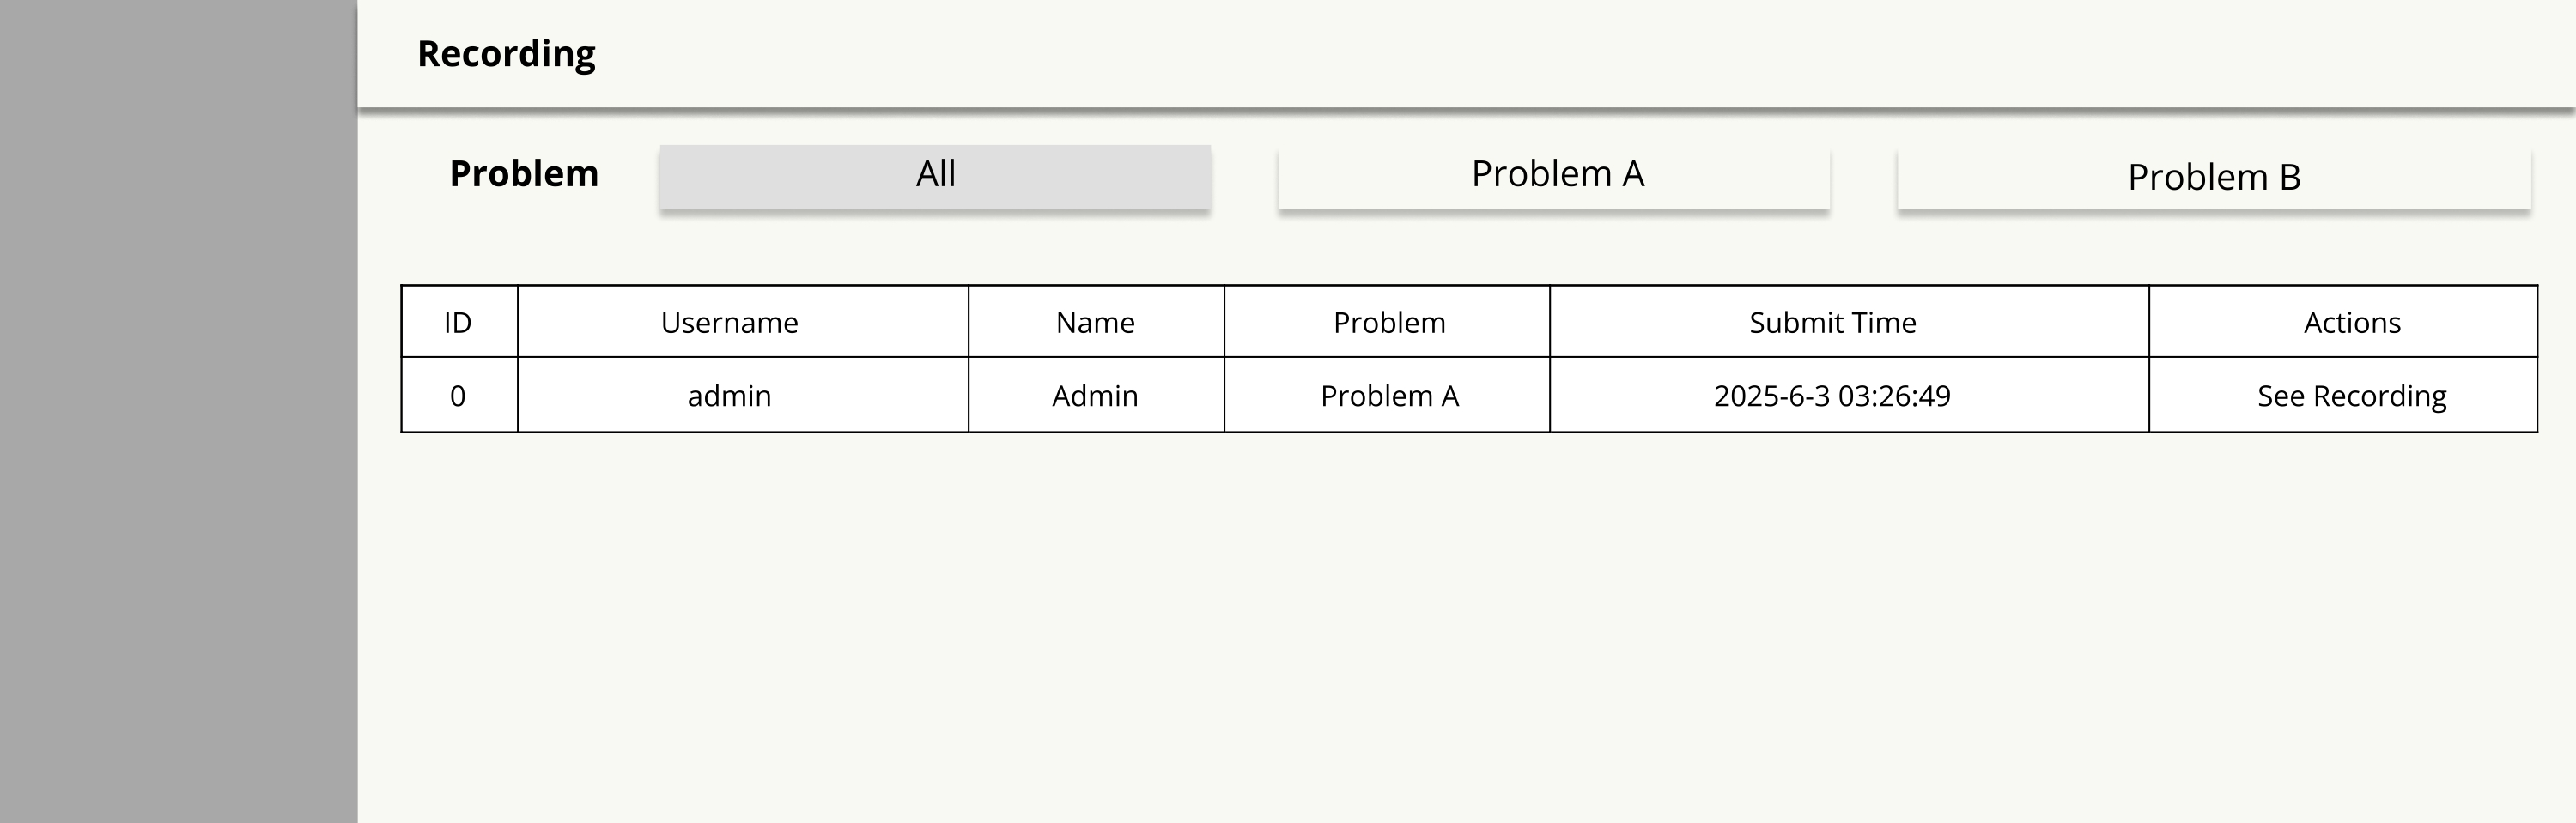
\includegraphics[width=0.75\textwidth]{design-recording-list.jpg}
    \caption{Rancangan Antarmuka Halaman Daftar Rekaman}
    \label{fig:4:1:listrec}
\end{figure}

\begin{figure}[H]
    \centering
    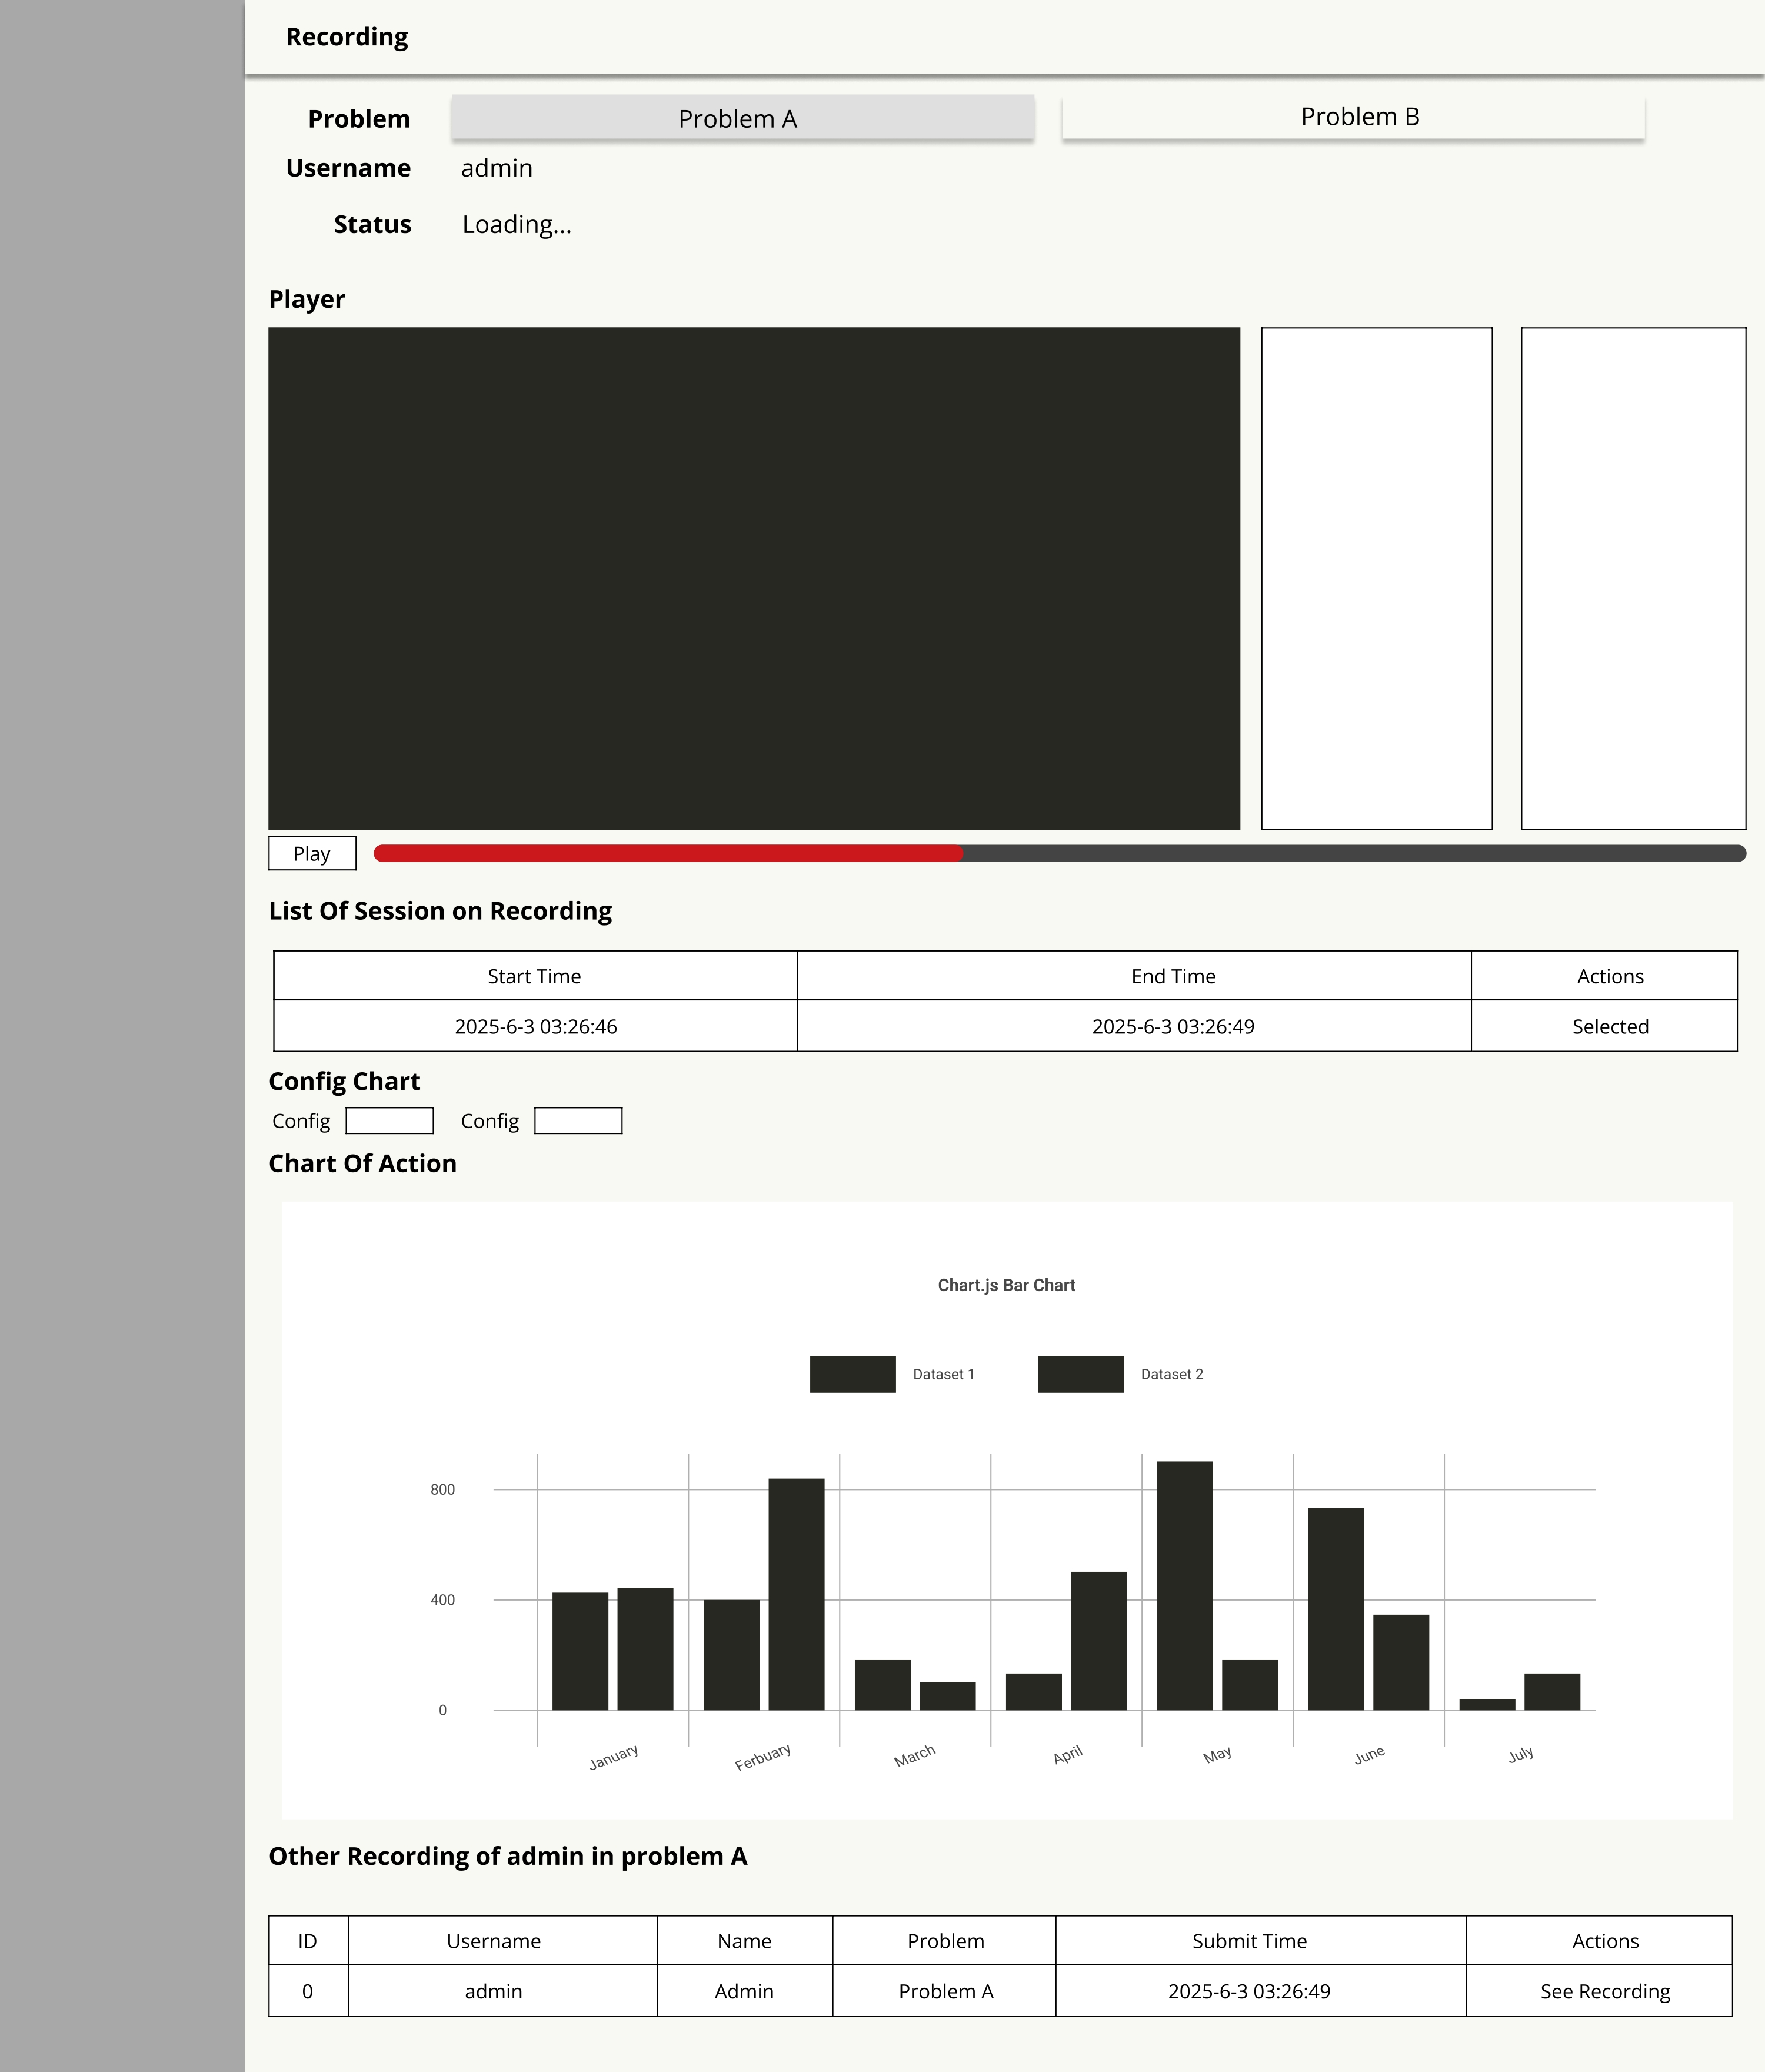
\includegraphics[width=0.75\textwidth]{design-recording.jpg}
    \caption{Rancangan Antarmuka Halaman Pemutaran Ulang}
    \label{fig:4:1:rec}
\end{figure}

\section{Rancangan Penyimpanan Rekaman}
\label{sec:4:2:storerekaman}

Rekaman yang akan disimpan akan berupa sebuah daftar \textit{event} yang terjadi. Dalam \textit{JavaScript}, daftar tersebut akan menjadi \textit{array} yang berisi \textit{event-event} yang terjadi. Rekaman juga akan menyimpan waktu dimana rekaman dimulai, awal kode yang ada dalam editor kode dan juga awal posisi kursor dalam IDE. Rekaman akan menjadi sebuah objek \mbox{\textit{JavaScript} yang berisi sebagai berikut:}

\begin{enumerate}
    \item \verb|timestart|: Waktu awal rekaman dimulai.
    \item \verb|start_value|: Isi awal dalam editor kode.
    \item \verb|start_cursor|: Posisi awal kursor dalam editor kode.
    \item \verb|events|: Daftar \textit{event} yang terjadi.
\end{enumerate}

\textit{Event} yang akan direkam juga membutuhkan beberapa data yang harus disimpan yaitu: waktu \textit{event} terjadi, \textit{event} yang terjadi, dan muatan \textit{event} yang terjadi. Maka \textit{event} juga akan disimpan dalam bentuk objek \textit{JavaScript}. Berikut merupakan format sebuah \textit{event}:

\begin{center}
    \verb|{time: <time>, event: <event>, payload: <payload>}|
\end{center}

Berikut merupakan penjelasan tentang format penyimpanan perekaman.

\begin{itemize}
    \item \verb|<time>| akan menunjukkan pada milidetik berapa event terjadi setelah waktu awal perekaman dimulai. sedangkan \verb|<event>| dan \verb|<payload>| merupakan data event yang terjadi.

    \item \verb|<event>| merupakan \textit{event} yang terjadi pada \verb|<time>|, contohnya adalah pengguna melakukan perubahan pada editor kode dengan menambahkan huruf `a', maka \textit{event} yang terjadi merupakan \textit{insert}. Semua event yang ditanggap akan dijelaskan pada sub Bagian \ref{sub:4:3:merekam}.

    \item \verb|<payload>| merupakan muatan \textit{event} yang terjadi. Muatan akan disesuaikan dengan \textit{event} yang terjadi. Sebagai contoh untuk event \textit{insert} di atas, maka isi dari \textit{event} tersebut adalah huruf `a', dan posisi kursor dalam editor kode dimana huruf tersebut dimasukkan.
\end{itemize}

Berikut contoh hasil untuk sebuah \textit{event insert} pada penjelasan di atas:

\begin{center}
    \verb|{time: 1203, event: "insert", payload: {data: "a", start: [10, 9]}}|
\end{center}

Penyimpanan rekaman juga akan disimpan pada direktori yang sama dengan penyimpanan kode submission seperti yang dijelaskan pada Bagian \ref{sub:3:1:penyimpanankode} dengan nama file \verb|record|.

\section{Rancangan Perubahan Kode}

Untuk mengimplementasikan fitur yang telah diusulkan pada Bagian \ref{sec:3:sistemusulan}, diperlukan beberapa perubahan pada kode sumber SharIF-Judge. Berikut merupakan rancangan untuk setiap fitur:

\subsection{Merekam perubahan atau event}
\label{sub:4:3:merekam}

Untuk menambahakan fitur ini, diperlukan perubahan pada bagian \textit{JavaScript} yaitu \verb|assets/js/|\\\verb|shj_submit.js| dalam halaman Submit. Dimana \textit{JavaScript} tersebut akan menjalankan perekaman secara otomatis saat pengguna memilih \textit{problem} yang ada dalam \textit{assignment} yang dipilih. Berikut merupakan \textit{event} yang akan ditangkap oleh \textit{JavaScript} dalam halaman Submit:

\begin{itemize}
    \item Perubahan isi kode pada editor kode.
    \item Perubahan posisi kursor pada editor kode.
    \item Perubahan fokus pada web page.
    \item Pergantian \textit{tab} dalam browser.
    \item Perubahan fokus pada PDF Viewer.
    \item Perubahan isi pada editor \textit{input} dalam IDE.
    \item Perubahan isi pada editor \textit{output} dalam IDE.
    \item Aksi men-\textit{Save}.
    \item Aksi men-\textit{Save \& Execute}.
    \item Aksi men-\textit{Save \& Submit}.
\end{itemize}

\subsection{Menyimpan rekaman}
\label{sub:4:3:menyimpanrekaman}

Fitur ini akan dilakukan setiap aksi menyimpan kode, menjalankan kode dengan tes kasus, dan mengumpulkan kode melalui IDE. Data rekaman juga akan disimpan ke dalam sistem dan \textit{database}. Untuk itu, perlu dilakukan perubahan sebagai berikut:

\begin{itemize}
    \item \textit{Controller} Submit:
          \begin{itemize}
              \item Fungsi \verb|save($type)|: \\
                    Fungsi ini akan diubah agar dapat menangani data rekaman yang dikirim oleh pengguna. Data tersebut akan disimpan dalam direktori yang sama dengan kode program.
              \item Fungsi \verb|_submit($data, $problem_id, $language, $user_dir)|: \\
                    Fungsi diubah agar untuk setiap \textit{submit}, rekaman dari \textit{save} sebelumnya akan diubah menjadi rekaman untuk \textit{submit} tersebut.
          \end{itemize}
    \item \textit{Assets} \verb|shj_submit.js|: \\
          Pada file \textit{assets} ini akan ditambahkan data rekaman yang dimuat ke dalam fungsi aksi menyimpan kode, menjalankan kode dengan tes kasus, dan mengumpulkan kode melalui IDE, rekaman juga akan disimpan ke dalam sistem.
\end{itemize}

\subsection{Melihat daftar rekaman}
\label{sub:4:3:melihatdaftarrekaman}

Untuk melihat semua daftar rekaman yang terjadi, maka dibutuhkannya \textit{database} untuk menyimpan dan mendapatkan daftar rekaman yang sudah disimpan dalam sistem. Setelah itu dibutuhkannya juga halaman baru dalam SharIF-Judge, maka perubahan yang dilakukan adalah sebagai berikut:

\begin{itemize}
    \item \textit{Controller} Submit:
          \begin{itemize}
              \item Fungsi \verb|save($type)|: \\
                    Fungsi ini menambahkan \textit{metadata} rekaman pengguna ke dalam \textit{database}. \textit{Metadata} yang dimaksud adalah \textit{id problem}, \textit{id assignment}, dan pengguna yang direkam. Metadata dalam database digunakan untuk mendapatkan daftar rekaman yang belum disubmit pada sebuah \textit{problem} dalam \textit{assignment} beserta dengan nama pengguna rekaman.
              \item Fungsi \verb|_submit($data, $problem_id, $language, $user_dir)|: \\
                    Perubahan untuk fitur melihat daftar rekaman akan menambahkan \textit{metadata} ke dalam \textit{database} sebagai daftar rekaman yang sudah di submit. \textit{Metadata} yang dimaksud adalah \textit{id problem}, \textit{id assignment}, dan pengguna yang direkam. Metadata dalam database digunakan untuk mendapatkan daftar rekaman yang sudah disubmit pada sebuah \textit{problem} dalam \textit{assignment} disertai dengan pengguna yang direkam.
          \end{itemize}
    \item \textit{Controller} Recording: \\
          Sebuah \textit{controller} baru yang menangani segala hal mengenai sistem pemutaran ulang dalam SharIF-Judge. Fungsi yang dibutuhkan agar fitur ini berjalan hanyalah fitur untuk menunjukkan daftar rekaman dalam sistem dengan mengambil data dari \textit{model} Recording dan menyimpannya dalam \textit{view} recording. Setelah itu, \textit{controller} akan menunjukkan \textit{view} tersebut kepada pengguna yang sudah login dan memiliki akses \textit{instructor} atau lebih tinggi.
          % \item Fungsi \verb|index()|:
          % \item Fungsi \verb|download_record()|:
    \item \textit{Model} Recording: \\
          Sebuah \textit{model} baru yang menangani segala hal mengenai penyimpanan dan pengambilan data rekaman dalam \textit{database}. Fungsi-fungsi yang direncanakan untuk diimplementasikan dalam \textit{model} Recording adalah sebagai berikut:
          \begin{itemize}
              \item Fungsi \verb|get_recording()|: \\
                    Fungsi digunakan untuk mendapatkan seluruh daftar rekaman dalam database. Fungsi ini dapat menyaring daftar rekaman berdasarkan \textit{assignment}, \textit{problem}, dan pengguna.
              \item Fungsi \verb|add_recording()|: \\
                    Fungsi ini digunakan untuk menyimpan sebuah rekaman ke dalam database.
          \end{itemize}
    \item \textit{View} \verb|Recording_list|: \\
          Sebuah \textit{view} baru yang menampilkan daftar rekaman yang ada dalam sistem. \textit{View} ini akan digunakan oleh \textit{Controller} Recording.
\end{itemize}

\subsection{Pemutaran ulang rekaman}

Untuk dapat memutar ulang rekaman diperlukan beberapa perubahan kode dalam SharIF-Judge. Berikut merupakan rencana perubahan kode dalam SharIF-Judge:

\begin{itemize}
    \item \textit{Controller} Recording: \\
          \textit{Controller} Recording merupakan sebuah \textit{controller} baru untuk menangani segala hal mengenai sistem pemutaran ulang dalam SharIF-Judge. Untuk fitur pemutaran ulang rekaman, diperlukan dua fungsi pada \textit{controller} yaitu sebagai berikut:
          \begin{itemize}
              \item Fungsi \verb|index()|: \\
                    Fungsi ini digunakan untuk menunjukkan \textit{view} \verb|Recording| kepada pengguna.
              \item Fungsi \verb|download_record()|: \\
                    Fungsi ini digunakan untuk mendapatkan \textit{file} rekaman dalam sistem. Fungsi ini akan dipanggil menggunakan AJAX dalam \textit{assets} \verb|Recording.js|.
          \end{itemize}
    \item \textit{Model} Recording: \\
          Sebuah \textit{model} baru yang menangani segala hal mengenai penyimpanan dan pengambilan data rekaman dalam \textit{database}. Fungsi yang dibutuhkan oleh fitur pemutaran ulang rekaman adalah fungsi \verb|get_recording()| untuk mendapatkan seluruh daftar rekaman sebuah pengguna dalam database berdasarkan \textit{problem} dan \textit{assignment}.
    \item \textit{View} \verb|Recording|: \\
          Sebuah \textit{view} baru yang menampilkan rekaman sebuah pengguna yang ada dalam sistem. \textit{View} ini akan digunakan oleh \textit{Controller} Recording.
    \item \textit{Assets} \verb|Recording.js|: \\
          \textit{Assets} \verb|Recording.js| merupakan sebuah \textit{assets} \textit{JavaScript} baru untuk digunakan oleh \textit{view} \verb|Recording| sebagai \textit{script} yang akan dijalankan oleh \textit{browser} pengguna.
\end{itemize}